\documentclass[12pt,a4paper]{report}
\usepackage{graphicx}
\usepackage{multicol}

%The below Section make chapter and its name to center of the page
\usepackage{blindtext}
\usepackage{xpatch}
\usepackage{mathptmx}
\usepackage{geometry}
 \geometry{
 right=25mm,
 left=25mm,
 top=25mm,
 bottom=25mm,
 }
 
\graphicspath{ {images/} }


\begin{document}
\begin{center}
\vspace{4cm}
{\Huge \textbf{QUADRUPED ROBOT}}\\

\vspace{2cm}
\Large PROJECT REPORT\\

\vspace{1.75cm}

Submitted by\\
\vspace{0.5cm}
\large Abdul Ahad\\
\large Atul Vyshnav R\\
\large Krishnanand K\\ 
\large Shinas Shaji\\
\vspace{1.5cm}
Under the supervision of\\
\large Dr. Sunil Kumar\\

\vspace{1cm}


\includegraphics[width=0.5\textwidth]{logo_rit}

\vspace*{\fill}
\end{center}

\begin{center}
\large Department of Electrical and Electronics Engineering\\
\large Govt. Rajiv Gandhi Institute of Technology, Kottayam\\
\large Velloor, Pampady, Kottayam - 686501\\
\end{center}

\newpage

\begin{center}
    \begin{center}   
        
\includegraphics[width=0.35\textwidth]{logo_rit}
    \end{center}
\vspace{0.5cm}
\large Department of Electrical and Electronics Engineering\\
\large Govt. Rajiv Gandhi Institute of Technology, Kottayam\\
\large Velloor, Pampady, Kottayam - 686501\\
\vspace{2 cm}

\textbf{\underline{CERTIFICATE}}\\
\vspace{0.5cm}
\end{center}
This is to certify that this report entitled “Quadruped Robot” submitted by  Mr. Abdul Ahad (Reg No: KTE18EE), Mr. Atul Vyshnav R (Reg No: KTE18EE), Mr. Krishnanand K (Reg No: KTE18EE040) and Mr. Shinas Shaji (Reg No: KTE18EE) to APJ Abdul Kalam Technological University in partial fulfillment of the requirements for the award of Degree of Bachelor of technology in Electrical and Electronics Engineering, is a bonafide record of the project carried out by them under our guidance and supervision. This report in any form has not been submitted to any other University or Institute for any purpose. 


\newpage
\begin{center}
     \Large  \textbf{ABSTRACT}\\
     \vspace{0.5cm}
    
\end{center}
Keywords: Quadruped, Autonomous, Path planning, Servo, Computer vision, Inverse Kinematics, LiDAR\\
\vspace{0.5cm}

Quadruped robots are highly afficient and advantageous when compared with other wheeled and 2 legged robots.The fact that it has 4 legs for locomotion creates extra possibilities of movement, stability and dynamic maneuvarability. Hence proving to be perfect for navigating complex terrains. Additionally the low center of gravity of these robots provide much more stability and balance to its movements. It's design and the gait pattern is inspired form that of animals.The project implements the movement functionalities of the quadruped and tackles the navigation and visual perception is done by the means of computer vision prgrammed in python for the purpose of Autonomous navigation. RaspberryPi is used as the main brain and Arduino Mega controls the actuators and the servo motors. Several Vision constraints are solved using path planning algorithms, stair detection, visual odometry etc. Inverse Kinematics is used to find the angles for the joints in the movement operation of the servos. This helps the robot for locomotion. Stereo Camera Setups, ultrasonic sensors and RPLiDAR is used for environment mapping and the data from these are used is the overall perception and navigation of the robot.


\newpage
\begin{center}
     \Large  \textbf{ACKNOWLEDGEMENT}\\
\end{center}
     \vspace{0.5cm}
     
     The successful completion of any task is incomplete and meaningless without giving any due credit to the people who made it possible without which the project would not have been successful and would have existed in theory.
     
     First and foremost, we are grateful to Dr. Johnson, HoD Electrical and Electronics Engineering Department, Dr. Prince Asok, Dr. Dolly, Dr. Shanifa Nisam and Prof. Peter K Abraham for their constant guidance and support. We would also like to thank our guide Dr. Sunil Kumar for his motivation and guidance in undertaking this endeavour.
     
     We would also like to take this moment to show our thanks and gratitude to one and all, who indirectly or directly have given us their hand in this challenging task. We feel happy and joyful and content in expressing our vote of thanks to all those who have helped us and guided us in presenting this project work for our Major project. Last, but never least, we thank our well-wishers, friends and parents for always being with us, in every sense and constantly supporting us in every possible sense whenever possible.

\vspace{2 cm}                        
\begin{multicols}{3}
\centering
\textbf{Dr. Johnson Mathew}\\
\textbf{Head of Department}\\
\vspace{0.3cm}


\textbf{Dr. Prince Asok}\\
\textbf{Coordinator}\\
\vspace{0.3cm}


\textbf{Dr. Sunil Kumar}\\
\textbf{Supervisor}\\
\vspace{0.3cm}
\end{multicols}





\newpage
\chapter{INTRODUCTION}
\section{Overview}

The necessity and requirements of different kinds of artificially intelligent robots are increasing day by day in the modern world. The latest innovations in technology are making possible for us to further develop in the different areas of human life. One of such up and rising sector is the robotic industry. 

In the world of robots, quadrupeds, or robots with 4 legs, are best equipped with the ability to maneuver complex terrain much faster and with enhanced stability. It follows the gait patterns of animals and are versatile in locomotion and movement. That is the sole intent behind the development of these kinds of beasts by robot enthusiasts around the world.

Mobile robots like quadrupeds have extensive application and potential to be one of the important innovations in the future of technology. Quadruped robots are superior in ability when commpared with wheeled and tracked robot due to its potential to explore in all the terrain like the human and animal. It also provides much more stability than a humanoid robots because of its 4 legged from that enables it to exploit the advantages of legged locomotion. The dynamic range of feet placement extends the reach and limits the constraints on directional movement. In addition to this, the low center of gravity accounts for enhanced balance and stability preventing the robot from toppling over in difficult circumstances.Hence reducing the damage and failure of the robot.Considering the dynamic and stable capabilities of a quadruped robot, we have taken inspiration from the immaculate development in the realm of Quadruped robots and have tried to recreate one of our own.

The robot works with information from stereo cam setups , LiDAR data and Even auxiliary sensors like the ultrasonic sensors  for tidy operation. Computer vision and Artificial Intellient techniques are incorporated with complex algorithms in the software side of things. 

\section{3D Modelling}

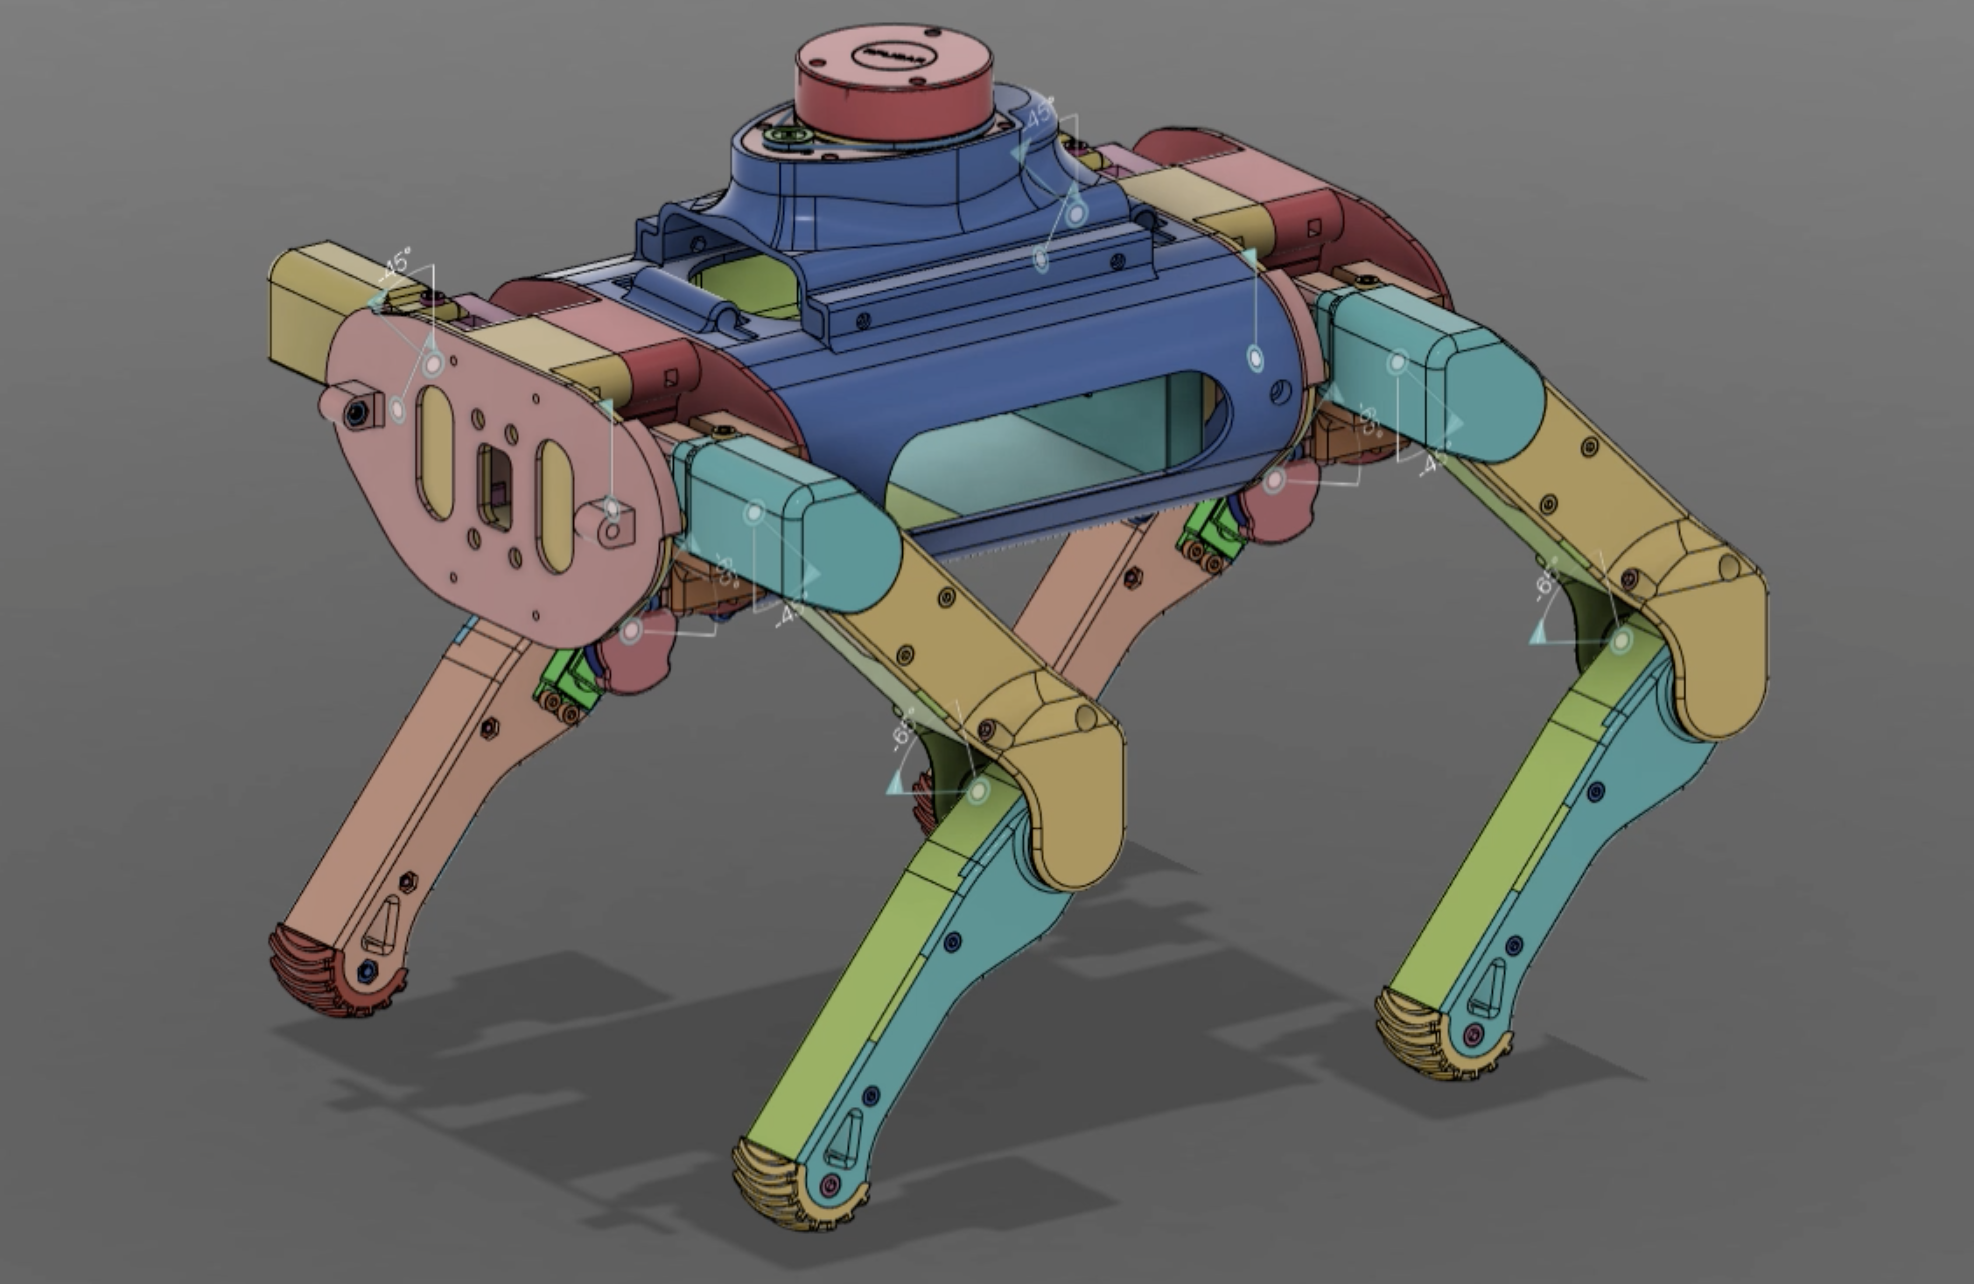
\includegraphics[width=0.5\textwidth]{orbv2F360}

\end{document}
